\section{Proposed NeST-Com Framework}
\subsection{System Model and Multiscale Representation}
We transmit an RGB image $x\in[0,1]^{256\times256\times3}$ through an additive white Gaussian noise channel,
\begin{equation}
 y=s+n,\qquad n\sim\mathcal{CN}(0,\sigma^2 I_N),
 \label{eq:channel}
\end{equation}
with nominal symbol energy $E_s=2$ and $\mathrm{SNR}=10\log_{10}(E_s/\sigma^2)$. The main configuration allocates $N=1024$ complex channel uses per image. In NeST-Com, a 12-bit profile ID is protected by CRC16 and a terminated rate-1/2 convolutional code, then transmitted using 68 BPSK symbols with constellation $\{\pm(1+j)\}$. The remaining 956 symbols carry the coded body. The profile identifies the actual source endpoint and modulation and coding scheme (MCS), enabling the receiver to interpret the body.

A frozen residual vector-quantized tokenizer produces token maps $q_1,\ldots,q_S$. We use $S=10$ scales with side lengths $(1,2,3,4,5,6,8,10,13,16)$ and a 4096-entry codebook. At each scale, the encoder quantizes the residual left by coarser scales. Let $L_s$ be the number of tokens in map $q_s$ and $C_s$ the codebook lookup, resizing, and residual transform to the common latent resolution. The complete latent is $f_q=\sum_{s=1}^S C_s(q_s)$, followed by image decoder $\Dc$. The tokenizer and VAR prior are frozen. $\Dc$ is fine-tuned on 20\,000 ImageNet training images using a fixed mixture of continuous, fully quantized, and prefix-completion-interpolated latents; its weights remain fixed during evaluation.

The frozen VAR predicts a scale from its complete coarser context:
\begin{equation}
 p_\theta(q_s\mid q_{<s})=\prod_{i=1}^{L_s}p_\theta(q_{s,i}\mid q_{<s}).
 \label{eq:prior}
\end{equation}
These probabilities define arithmetic-coding cumulative distribution functions (CDFs) at both ends of the link~\cite{arithmetic}. Fig.~\ref{fig:system} connects the representation, digital frame, and receiver completion.

\begin{figure*}[t]
\centering
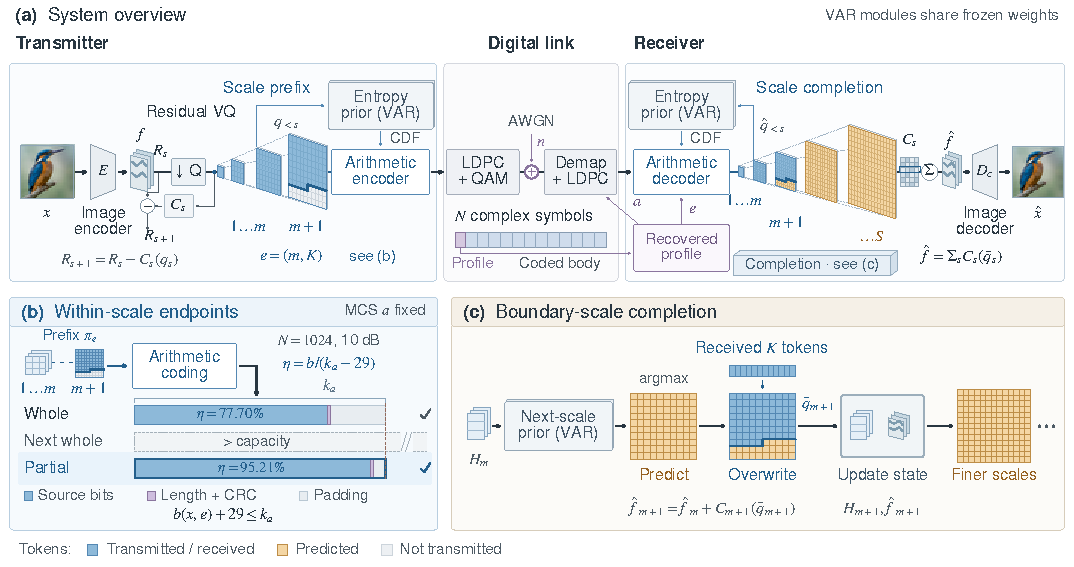
\includegraphics[width=\textwidth]{figure1.pdf}
\caption{NeST-Com. (a) The transmitter entropy-codes a next-scale token prefix with endpoint $e=(m,K)$ using CDFs from a frozen VAR. The receiver rebuilds these CDFs from decoded coarse-scale tokens $\hat q_{<s}$; the recovered profile gives $e$ and MCS $a$. (b) The terminated stream of length $b(x,e)$, a 13-bit length field, and CRC16 must fit within the LDPC information length $k_a$. Mean source-bit utilization rises from 77.70\% to 95.21\% (500 images, $N=1024$, 10~dB). WHOLE/PARTIAL bars use these measured means. (c) The $K$ received boundary tokens overwrite the VAR predictions; the merged map $\tilde q_{m+1}$ conditions finer scales. $H_m$ is the VAR state after scale $m$; $C_s$ comprises codebook lookup, resizing, and a scale-dependent residual transform.}
\label{fig:system}
\end{figure*}

\subsection{Budget-Adaptive Within-Scale Prefix Transmission}
For $m<S$, an endpoint $e=(m,K)$ specifies the transmitted prefix
\begin{equation}
 \pi_e=(q_1,\ldots,q_m,q_{m+1,1:K}),
 \label{eq:prefix}
\end{equation}
where positions within a map follow raster order. $K=0$ denotes a complete-scale endpoint. For a partial boundary with $L=L_{m+1}$, the implemented candidates are
\begin{equation}
 K\in\{\lfloor L/4\rfloor,\lfloor L/2\rfloor,\lfloor3L/4\rfloor\}.
 \label{eq:endpoints}
\end{equation}
We allow partial endpoints after scales $m=4,\ldots,9$. Their resolution is one quarter of a scale, with integer floors when token counts are not divisible by four. The complete representation is $e=(S,0)$ with $\pi_e=(q_1,\ldots,q_S)$ and needs no boundary completion.

For MCS $a=(M,r)$, the 956 body symbols carry $n_a=956\log_2 M$ coded bits, and the LDPC information length is $k_a=\lfloor rn_a\rfloor$. Let $b(x,e)$ denote the actual bit length after arithmetic-code termination. A feasible prefix satisfies
\begin{equation}
 b(x,e)+29\leq k_a,\qquad \eta(x,e)=\frac{b(x,e)}{k_a-29},
 \label{eq:budget}
\end{equation}
where 29 bits comprise a 13-bit stream-length field and a 16-bit cyclic redundancy check (CRC). Remaining information positions are zero-padded before body LDPC encoding, using the 5G NR code and rate-matching procedures~\cite{nr}, and quadrature amplitude modulation (QAM).

Offline calibration selects an SNR-specific target endpoint, MCS, and ordered fallback chain by maximizing the mean DINOv2 cosine similarity between source and reconstructed images on a calibration set~\cite{dinov2}. For each image, the transmitter arithmetic-codes the target prefix and moves to earlier legal endpoints until~\eqref{eq:budget} holds, keeping the selected MCS fixed. The protected profile records the resulting endpoint. Checking the terminated length accounts for image-dependent entropy and coding overhead. Quarter-scale endpoints provide intermediate choices when the next whole scale exceeds capacity.

We report the source-wise mean of $\eta$. At 10~dB, $k_a=2549$ leaves 2520 source bits; complete-scale and within-scale endpoint sets use 77.70\% and 95.21\% of this capacity, respectively. Finite endpoint spacing still leaves padding, as illustrated in Fig.~\ref{fig:system}(b).

\subsection{Prefix-Constrained Reconstruction}
A reception is rejected if the protected profile fails its CRC or catalogue check, the body CRC, declared length, or known padding is invalid, or arithmetic-source parsing fails. The receiver then outputs a fixed gray image.

For an accepted reception, the receiver arithmetic-decodes $\pi_e$. Before decoding each transmitted scale, it reconstructs the CDFs from already decoded complete coarser maps $\hat q_{<s}$. This reproduces the transmitter's probability model without transmitting CDFs. At the boundary scale, VAR predicts a full map from $\hat q_{\leq m}$. Denoting its deterministic argmax prediction by $q^{\mathrm{pred}}_{m+1}$, the receiver forms
\begin{equation}
 \tilde q_{m+1,i}=\begin{cases}
 \hat q_{m+1,i},&i\leq K,\\
 q^{\mathrm{pred}}_{m+1,i},&i>K.
 \end{cases}
 \label{eq:overwrite}
\end{equation}
The merged map updates the accumulated latent and VAR state before prediction advances. Every received token thus contributes to reconstruction and conditions finer scales. For complete received scales, $\tilde q_s=\hat q_s$; at the boundary, it follows~\eqref{eq:overwrite}; for untransmitted finer scales, it is the argmax prediction. The output is
\begin{equation}
 \hat x=\Dc\!\left(\sum_{s=1}^S C_s(\tilde q_s)\right).
 \label{eq:reconstruction}
\end{equation}
This predict--overwrite--advance procedure makes a partial map a valid context for the same next-scale prior used by the entropy coder.
